\documentclass{ctexart}
\usepackage{babel}
\usepackage{anyfontsize}
\usepackage[letterpaper,top=2cm,bottom=2cm,left=3cm,right=3cm,marginparwidth=1.75cm]{geometry}
\usepackage{amsmath, amssymb}
\usepackage{graphicx}
\usepackage{floatrow}
\usepackage[colorlinks=true, allcolors=blue]{hyperref}
\usepackage{enumitem}
\usepackage{longtable}
\usepackage{listings}
\usepackage{xcolor}
\definecolor{teal}{RGB}{0,128,128}
\setlist[itemize]{noitemsep}
\lstset{
    basicstyle          =   \sffamily,          % 基本代码风格
    keywordstyle        =   \bfseries,          % 关键字风格
    commentstyle        =   \rmfamily\itshape,  % 注释的风格,斜体
    stringstyle         =   \ttfamily,  % 字符串风格
    flexiblecolumns,                % 别问为什么,加上这个
    numbers             =   left,   % 行号的位置在左边
    showspaces          =   false,  % 是否显示空格,显示了有点乱,所以不现实了
    numberstyle         =   \zihao{-5}\ttfamily,    % 行号的样式,小五号,tt等宽字体
    showstringspaces    =   false,
    captionpos          =   t,      % 这段代码的名字所呈现的位置,t指的是top上面
    frame               =   lrtb,   % 显示边框
}

\lstdefinestyle{Python}{
    language        =   Python, % 语言选Python
    basicstyle      =   \zihao{-5}\ttfamily,
    numberstyle     =   \zihao{-5}\ttfamily,
    keywordstyle    =   \color{blue},
    keywordstyle    =   [2] \color{teal},
    stringstyle     =   \color{magenta},
    commentstyle    =   \color{red}\ttfamily,
    breaklines      =   true,   % 自动换行,建议不要写太长的行
    columns         =   fixed,  % 如果不加这一句,字间距就不固定,很丑,必须加
    basewidth       =   0.5em,
}

\title{\textbf{数据科学导论实验报告}}
\author{吕思翰\ 来泽远\ 曹宸瑞}

\begin{document}

\maketitle

% \tableofcontents
% \newpage

% \ctexset{abstractname=摘要}
% \begin{abstract}

% \end{abstract}

\section{比赛名称}

Predict CO2 Emissions in Rwanda(预测卢旺达二氧化碳排放量)

\section{成员}

\begin{itemize}
      \item 吕思翰 PB21000144
      \item 来泽远 PB21000164
      \item 曹宸瑞 PB21020659
\end{itemize}

\section{问题定义}

\subsection{Predicting CO2 Emissions}

准确监测碳排放能力是应对气候变化的重要步骤。精确的碳排放数据使研究人员和政府能够了解碳排放的来源和模式。尽管欧洲和北美已经建立了广泛的地面碳排放监测系统,但在非洲可用的系统相对较少。本任务要求参赛选手依据过往二氧化碳排放数据预测未来的排放数据。

\subsection{Dataset}

从卢旺达多个地区挑选了大约497个独特的地点,分布在农田、城市和发电厂周围。这次比赛的数据是按时间划分的;训练数据中包含2019 - 2021年的二氧化碳排放数据,任务是预测2022年至11月的二氧化碳排放数据。

\subsection{Evaluation}

本次比赛的评价指标是均方根误差(RMSE)。RMSE是预测值和实际值之间差异的平方的平均值的平方根。RMSE的值越低,表示模型的预测能力越好。RMSE定义为:

\[
      RMSE=\sqrt{\frac{1}{N}\sum\limits_{i=1}^{N}(y_i-\hat y_i)^2}.
\]

其中 $y_i$ 是真实值,$\hat y_i$ 是预测值,$N$ 是样本数量。

\section{数据分析}

\subsection{数据概览与特性}

训练集的基本信息如下。

\begin{table}[h]
      \centering
      \caption{数据集概览}
      \begin{tabular}{llll}
            \hline
            \#       & Column                                                     & Non-Null Count & Dtype            \\ \hline
            0        & \texttt{ID\_LAT\_LON\_YEAR\_WEEK}                          & 79023 non-null & \texttt{object}  \\
            1        & \texttt{latitude}                                          & 79023 non-null & \texttt{float64} \\
            2        & \texttt{longitude}                                         & 79023 non-null & \texttt{float64} \\
            3        & \texttt{year}                                              & 79023 non-null & \texttt{int64}   \\
            4        & \texttt{week\_no}                                          & 79023 non-null & \texttt{int64}   \\
            5        & \texttt{SulphurDioxide\_SO2\_column\_number\_density}      & 64414 non-null & \texttt{float64} \\
            6        & \texttt{SulphurDioxide\_SO2\_column\_number\_density\_amf} & 64414 non-null & \texttt{float64} \\
            \ldots{} &                                                            &                &                  \\
            74       & \texttt{Cloud\_solar\_zenith\_angle}                       & 78539 non-null & \texttt{float64} \\
            75       & \texttt{emission}                                          & 79023 non-null & \texttt{float64} \\
            \hline
      \end{tabular}
\end{table}

\begin{itemize}
      \item 数据集共有 79023 行,76 列,其中 75 列为特征,1 列为预测值。
      \item 只有数字特征特征(不包括用于索引的特征)。
      \item 训练数据在 2019-2021 年间测量。% ?
      \item 除经纬度外其余值均为 \texttt{float64},不需要做额外数据处理。
      \item 部分测试量包含空值,可以进行缺失值处理。
      \item 可用作索引的值有 \texttt{latitude},\texttt{longitude},\texttt{year} \texttt{week\_no},需预测值为 \texttt{emission}
      \item 其余特征可以分类为 \texttt{CarbonMonoxide},\texttt{Cloud}, \texttt{Formaldehyde},\texttt{NitrogenDioxide},\texttt{Ozone},\texttt{SulphurDioxide},\texttt{UvAerosolIndex},\texttt{UvAerosolLayerHeight}。
\end{itemize}

\subsection{特征分析}

\subsubsection{年份与周数}

首先我们考虑排放量与时间的关系。我们将年份和周数相关联作为日期,作出总排放量关于日期的折线图,得到结果如下图\ref{fig:2}。(红线划分了2019-2021年的数据)

\begin{figure}[H]
      \centering
      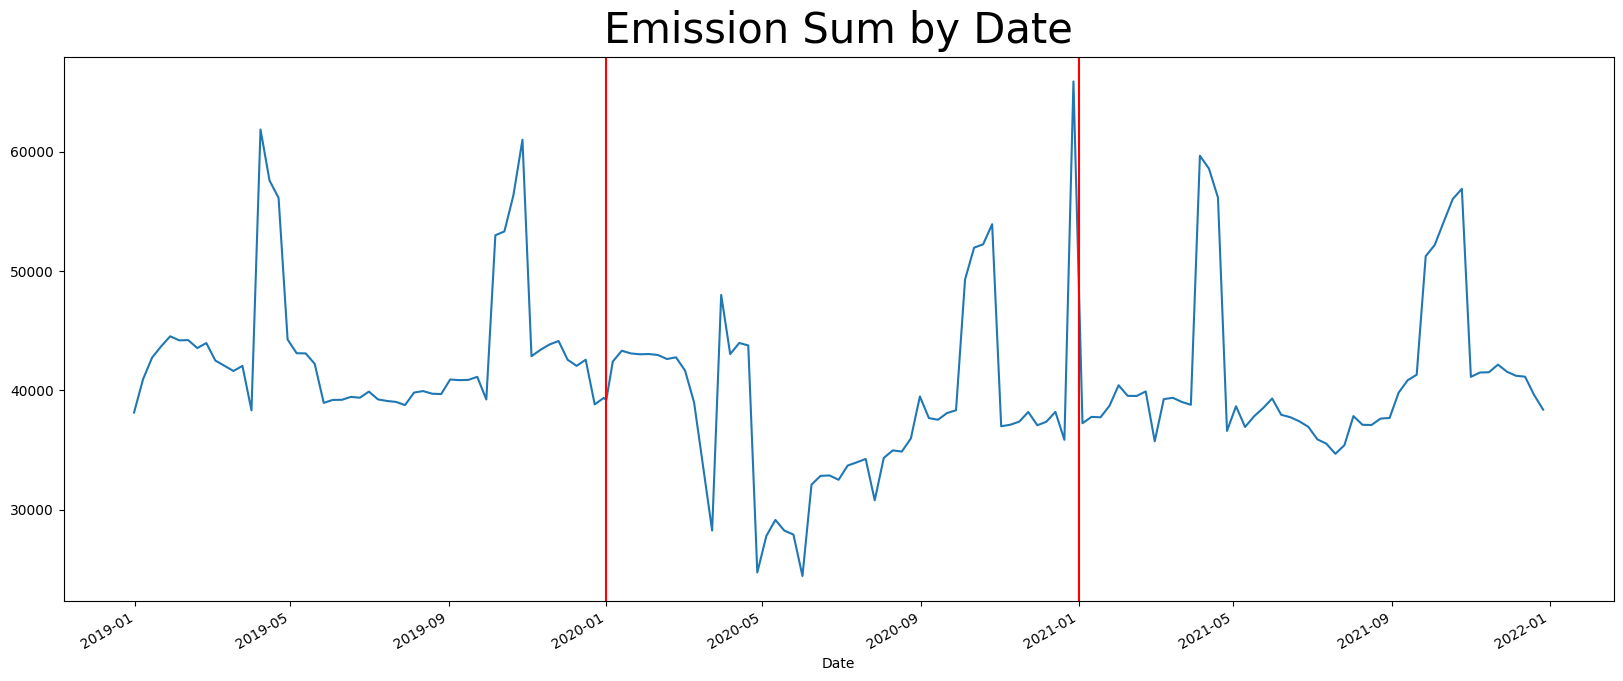
\includegraphics[width=1\textwidth]{output2.png}
      \caption{\label{fig:2}排放量关于日期的折线图}
\end{figure}

可以看出,排放量随时间的变化呈现出一定的周期性,因此我们认为年份和周数对于预测二氧化碳排放量有一定的参考价值。我们将年份和周数作为特征之一加入模型。

但是,值得注意的是,由于新冠病毒的影响,2020年的数据与其他年份的数据有较大的差异,后续需要针对2020年的数据进行特殊处理。

我们将2019与2021年的数据平均后,作图得到排放量关于月份的折线图,结果如图 \ref{fig:3}。

\begin{figure}[H]
      \centering
      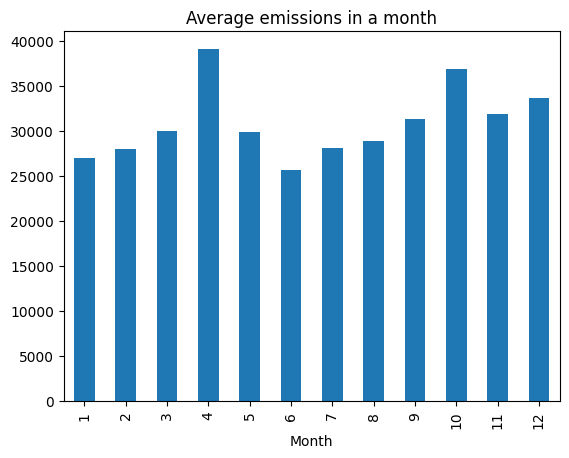
\includegraphics[width=1\textwidth]{output3.png}
      \caption{\label{fig:3}排放量关于月份的折线图}
\end{figure}

结合两图可以发现,一年内某几个特殊的月份具有较高的排放量,这可能与人类生产活动习惯相关。对于同一个地点,周数(月份)与排放量具有较高的相关性,且关于年份呈现周期变化。这对于数据处理有一定的借鉴意义。

\subsubsection{经纬度}

首先,我们将每个地区的排放量求和,以其排放量为半径,以其经纬度为圆心,按照排放量高低标记颜色从浅至深,作出排放量关于经纬度的分布图,结果如图 \ref{fig:9}。

\begin{figure}[H]
      \centering
      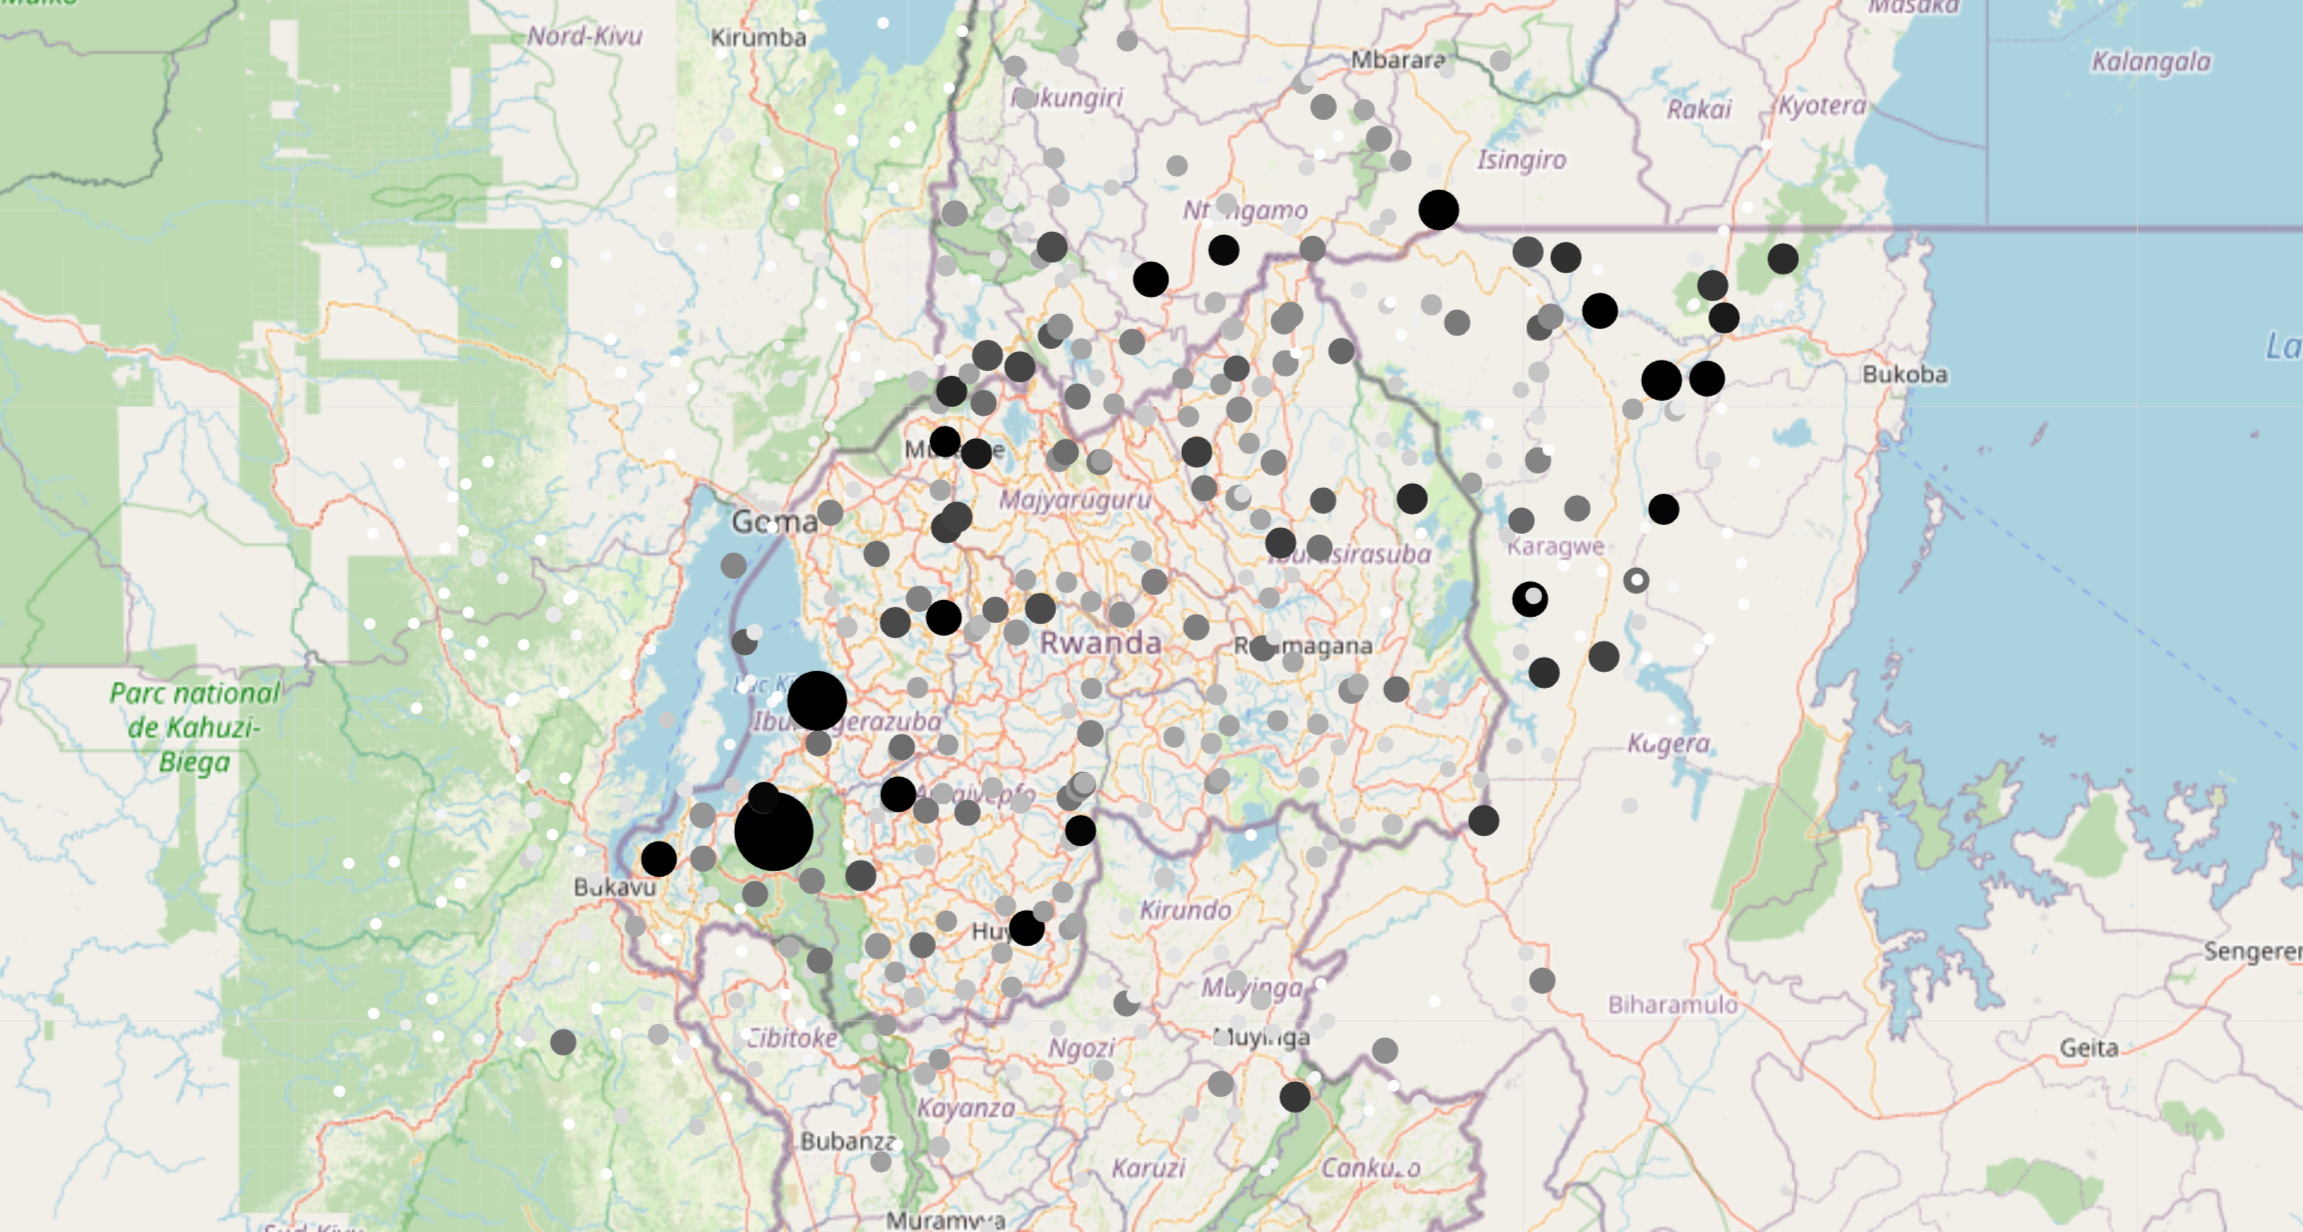
\includegraphics[width=1\textwidth]{output9.png}
      \caption{\label{fig:9}排放量关于经纬度的分布图}
\end{figure}

和城市聚集类似,几个距离较近的采样点,他们的碳排放量也是相近的,并且不难发现大部分采样点较为密集,这为使用聚类提供了数据支持。在模型中,可以使用距离相近的采样点的数据来相互预测。

\subsubsection{关于时间和空间的总结}

\begin{itemize}
      \item 共有497个不同位置的排放数据。
      \item 排放量与季节有很强的依赖性。
      \item 有2个位置的排放量特别大。
      \item 测试集与训练集位置相同。
      \item 碳排放量有强周期性与聚集效应。
\end{itemize}

此外,我们考察不同地点碳排放的变化,作出各地点以年为单位的碳排放量变化如图 \ref{fig:5}。

\begin{figure}[H]
      \centering
      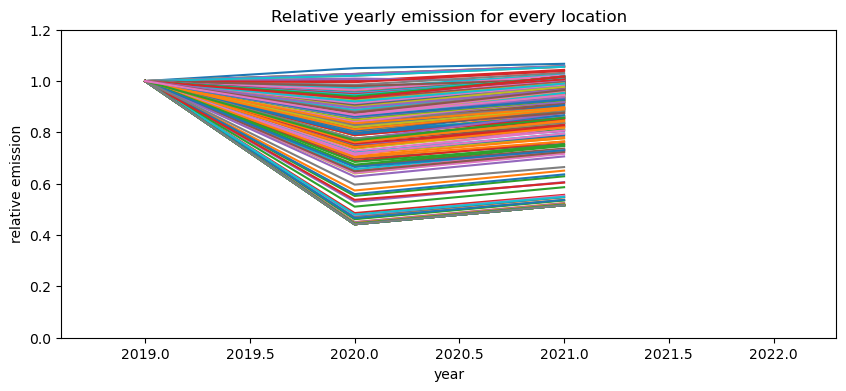
\includegraphics[width=1\textwidth]{output5.png}
      \caption{各地点排放量关于年份的折线图}
      \label{fig:5}
\end{figure}

我们将每一年的碳排放除以2019年的碳排放,作为相对值。若排除新冠的影响,对于绝大部分地点,其碳排放是较为稳定的,在某一个基准附近存一定浮动(多为上升)。而对于这个基准值,经纬度是与其强相关的。

作出各个地点以周为单位的碳排放量变化如图 \ref{fig:8}。

\begin{figure}[H]
      \centering
      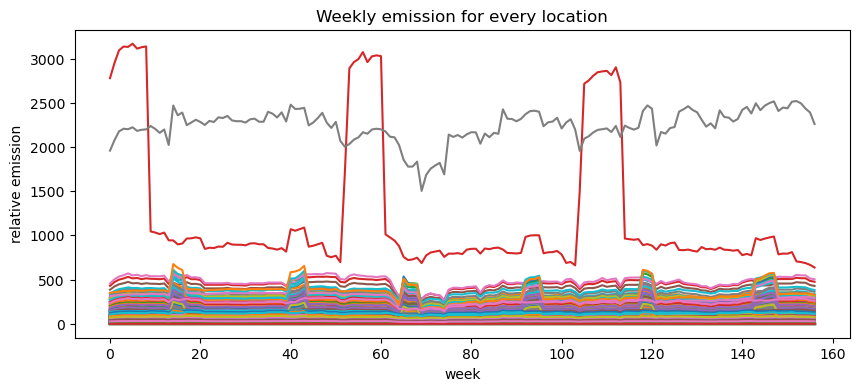
\includegraphics[width=1\textwidth]{output8.png}
      \caption{各地点排放量关于周数的折线图}
      \label{fig:8}
\end{figure}

作出各个地点每周碳排放量相比第0周的变化如图 \ref{fig:6}。

\begin{figure}[H]
      \centering
      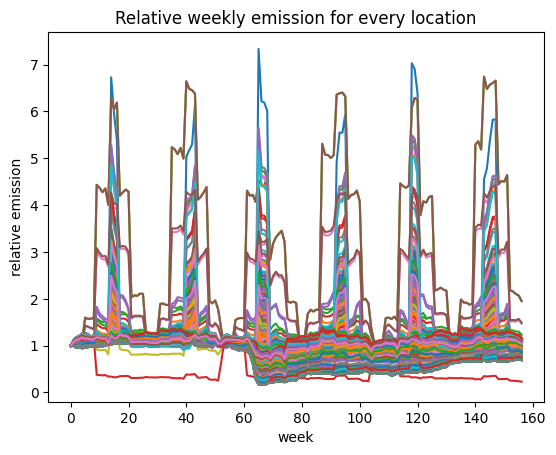
\includegraphics[width=1\textwidth]{output6.png}
      \caption{各地点每周碳排放量相比第0周的折线图}
      \label{fig:6}
\end{figure}

综合以上信息,可以总结一些预处理和建模的思路。
\begin{itemize}
      \item 年份、周数、经纬度都要作为特征加入模型。对于将绝对周数(0-160),我们不将其作为特征加入,原因是年内周数更有效地体现了周期性,而年份体现了新冠病毒影响下的趋势。
      \item 对于新冠影响,可以考虑修正2020的数据并且对预测值按一定比例提高,可以更有效地还原人类恢复生产的过程。
      \item 由于强周期性和聚集效应,可以使用聚类的方法,对于同一类的数据,可以使用相似的数据进行预测。
      \item 由于提供的年份较少以及新冠影响,对于年份的趋势变化的预测较为困难,应该避免过拟合。
\end{itemize}

\subsubsection{气象数据}

除了上述特征外,数据集还给出了大量的气象数据,包括二氧化硫(SO2)、一氧化碳(CO)、二氧化氮(NO2)、甲醛(HCHO)、臭氧(O3)、紫外线气溶胶、云等物质的方位角、天顶角、深度、角度、密度、压力、温度、反射率等信息。我们认为这些信息对于预测二氧化碳排放量有一定的参考价值。以下是对这些特征的分析。

以2020年 \texttt{SulphurDioxide\_SO2\_column\_number\_density} 为例,计算其与 \texttt{emission} 的相关系数并作出散点图。

得到结果如下:

\begin{center}
      Pearson correlation: -0.013960940599134839

      Spearman correlation: -0.06904123013729443
\end{center}


\begin{figure}[H]
      \centering
      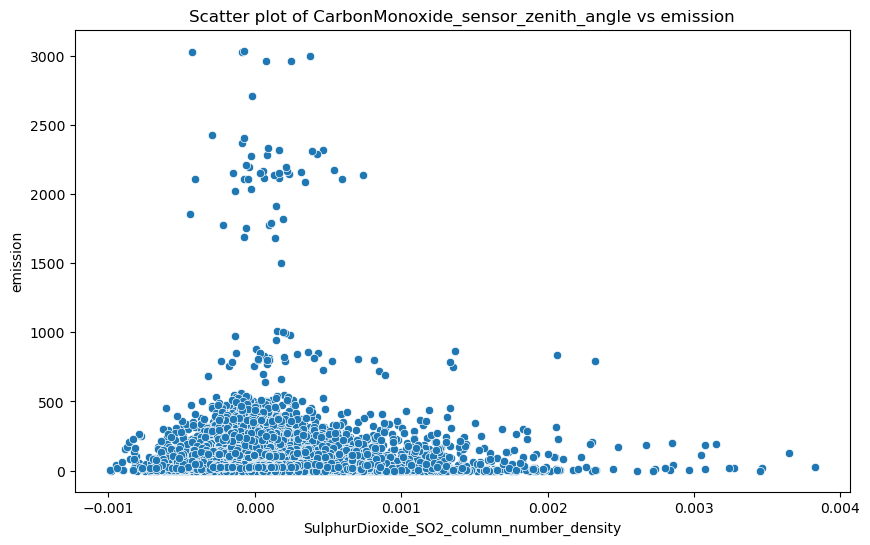
\includegraphics[width=1\textwidth]{output1.png}
      \caption{\texttt{SulphurDioxide\_SO2\_column\_number\_density} 与 \texttt{emission} 的散点图}
      \label{fig:1}
\end{figure}

可以看出,这两者之间的相关性非常小,因此我们认为 \texttt{SO2\_column\_number\_density} 数据对于预测二氧化碳排放量的影响可以忽略不计。

我们还对其他气象数据进行了类似的分析,但并没有出现与 CO2 有较大相关性的数据。初步分析后,我们认为这些气象数据与 CO2 排放量之间可能没有明显关系,理由如下:

\begin{itemize}
      \item 卢旺达是一个直径200公里的小国,每天都有邻国的空气取代卢旺达的整个大气。即使卢旺达所产生的各种气体之间有一定的相关性,也会被邻国的空气所影响。
      \item 二氧化碳排放来自不同的部门(地面交通、空中交通、供暖、发电、工厂等),而这些部门并不一定排放与 CO2 成比例的NO2、CO、SO2等气体。我们认为只在特定区域如工厂,CO2可能会与SO2等成正比例关系。
\end{itemize}

因此,我们借用排放量地图进行分析,对排放量最多的地点测量得到的数据进行相关性分析。有理由相信,如果CO2主要来自工厂,会同时产生等比例的大量SO2、CO等气体。以2021年 \texttt{CarbonMonoxide\_CO\_column\_number\_density} 为例,得到结果如下:

\begin{center}
      Pearson correlation: -0.0016211411671317282

      Spearman correlation: 0.002390506275078972
\end{center}

\begin{figure}[H]
      \centering
      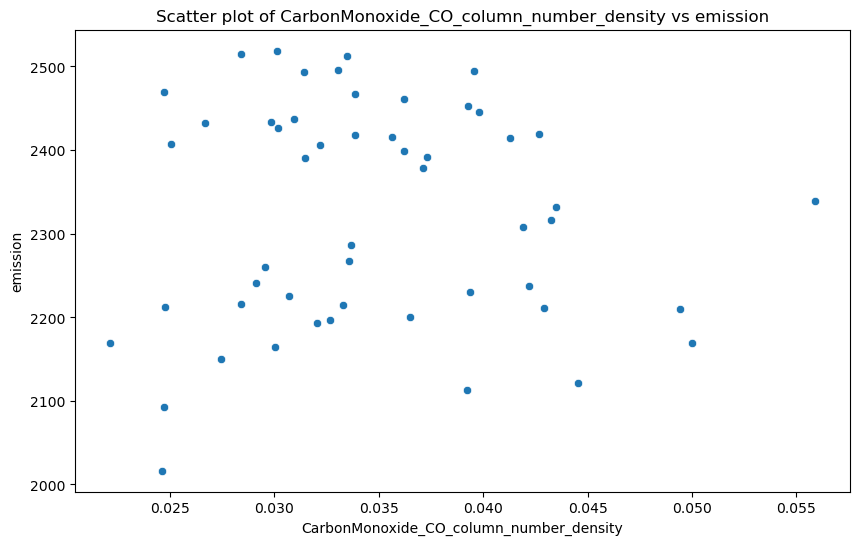
\includegraphics[width=1\textwidth]{output7.png}
      \caption{\texttt{CarbonMonoxide\_CO\_column\_number\_density} 与 \texttt{emission} 的散点图}
      \label{fig:7}
\end{figure}

我们无法得出该气体与CO2排放量之间有明显的相关性。类似的,我们对该地点的其他气象数据进行了计算,也未能分析出得到更多有价值的信息。

\subsubsection{权重量化}

我们在未经处理的数据中直接使用随机森林模型训练,得到的特征权重如下:

\begin{figure}[H]
      \centering
      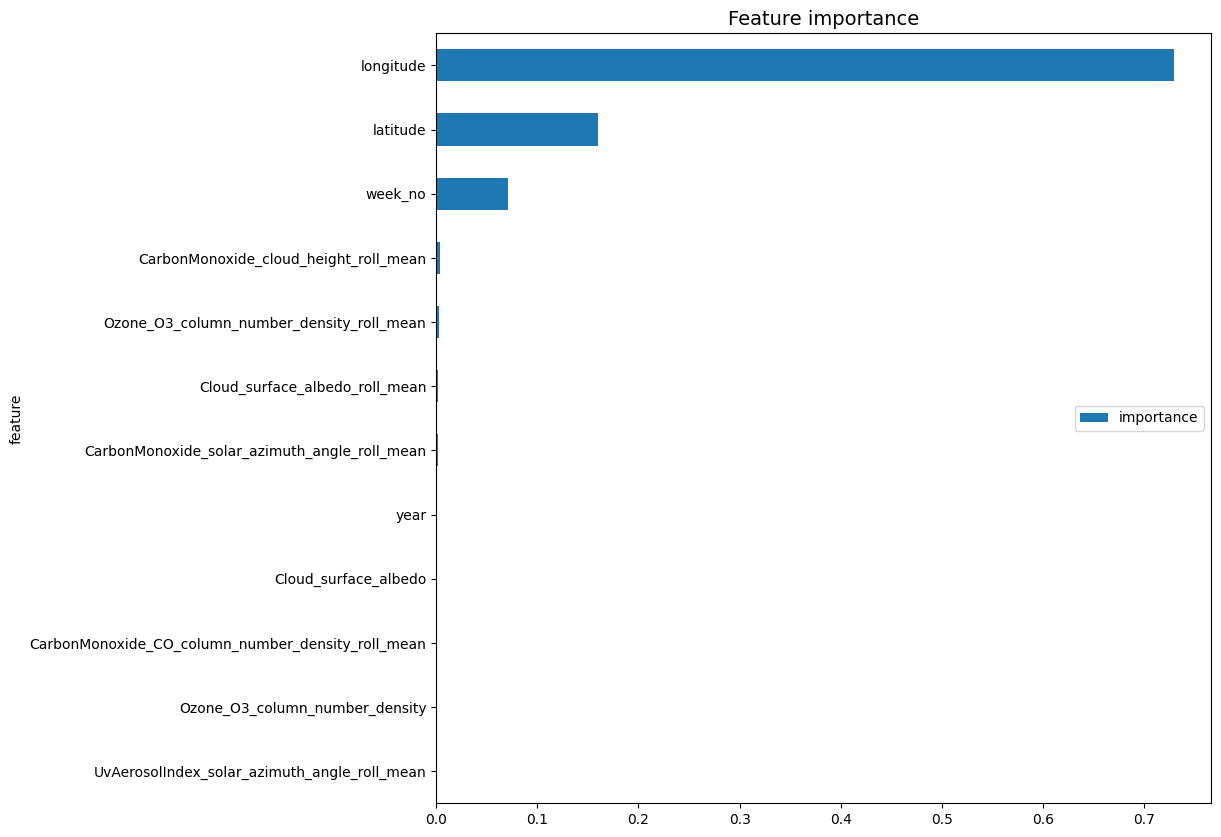
\includegraphics[width=0.9\textwidth]{output11.png}
      \caption{特征权重}
      \label{fig:11}
\end{figure}

可以看出,经纬度的权重较大,周数次之,年份权重虽小但是需要反应新冠趋势,无法舍弃。而其他气象数据的权重和我们先前的预测是相吻合的,与排放量的相关性较小。虽然该权重可能存在一定误差,但是有参考价值,我们后续的工作也将主要围绕时间和空间的特征进行。

\subsection{数据预处理}

\subsubsection{缺失值处理}

在数据预处理阶段,缺失值处理是一个重要的步骤。缺失值可能会导致统计分析的结果出现偏差,或者使得机器学习算法无法正确地工作。

使用 \verb|train.isnull().sum()| 可以查看训练集每一列的缺失值数量,结果如表 \ref{tab:1} 所示。

\begin{table}[h]
      \centering
      \caption{缺失值概览}
      \label{tab:1}
      \begin{tabular}{lc}
            \hline
            Column                                                                & Non-Null Count \\ \hline
            \texttt{UvAerosolLayerHeight\_aerosol\_height}                        & 78584          \\
            \texttt{UvAerosolLayerHeight\_solar\_zenith\_angle}                   & 78584          \\
            \texttt{UvAerosolLayerHeight\_solar\_azimuth\_angle}                  & 78584          \\
            \ldots{}                                                              &                \\
            \texttt{NitrogenDioxide\_tropopause\_pressure}                        & 18320          \\
            \texttt{NitrogenDioxide\_stratospheric\_NO2\_column\_number\_density} & 18320          \\
            \texttt{NitrogenDioxide\_NO2\_slant\_column\_number\_density}         & 18320          \\
            \ldots{}                                                              &                \\
            \texttt{SulphurDioxide\_SO2\_column\_number\_density\_15km}           & 14609          \\
            \texttt{SulphurDioxide\_solar\_zenith\_angle}                         & 14609          \\
            \texttt{SulphurDioxide\_solar\_azimuth\_angle}                        & 14609          \\
            \ldots{}                                                              &                \\
            \hline
      \end{tabular}
\end{table}

虽然某些机器学习算法,如决策树和随机森林,可以直接处理缺失值,但由于后续模型还未确定,故还是在此对缺失值进行处理。对于缺失值较多的列,如 \texttt{UvAerosolLayerHeight},缺失率达到 99\%,我们可以考虑直接删除。对于缺失值较少的列,我们可以考虑使用均值填充,或分组后使用邻近非缺失值填充,代码如下:

\begin{lstlisting}[style=Python]
      numeric_cols = train.columns.drop("ID_LAT_LON_YEAR_WEEK")
      train[numeric_cols] = train[numeric_cols].fillna(train[numeric_cols].mean())
\end{lstlisting}

对于测试集,我们可以进行类似缺失值处理操作。

\subsubsection{异常值处理}
2020年的数据受到新冠病毒影响,为异常数据。我们尝试了三种方法,一种为直接舍弃2020年以及2019末和2021初的数据;一种为将2020年的数据按照2019和2021的平均值上调一定幅度;一种为为2020年的数据加入一个特征。

\subsubsection{数据归一化}

数据归一化是一种常用的数据预处理技术,用于将数据转换到一个公共的尺度。这种技术在机器学习和数据挖掘中非常常见,因为许多算法(如神经网络)对输入数据的尺度和分布有一定的假设。

数据归一化通常涉及将数值特征缩放到一个固定的范围(如0到1),或者将它们转换为具有零均值和单位方差的值。这样可以确保所有特征在模型训练过程中具有相同的重要性,而不会因为它们的尺度不同而被赋予不同的权重。

可以使用 \texttt{sklearn.preprocessing} 模块中的 \texttt{MinMaxScaler} 或 \texttt{StandardScaler} 类来进行数据归一化,代码如下:

\begin{lstlisting}[style=Python]
      from sklearn.preprocessing import StandardScaler
      scaler = StandardScaler()
      scaler.fit(train)
      train = scaler.transform(train)
      test = scaler.transform(test)
\end{lstlisting}

\subsubsection{到卢旺达中心的距离}
我们认为CO2排放量与到卢旺达中心的距离有一定的相关性,因此我们计算了每个地点到卢旺达中心的距离,并将其作为特征之一加入模型。

\subsubsection{笛卡尔坐标转换}
我们还发现,在对坐标进行笛卡尔坐标转换后,排放量与坐标的关系较为明显,因此我们将对坐标旋转 15° 和 30° 的笛卡尔坐标分别作为特征加入模型,具体代码如下:

\begin{lstlisting}[style=Python]
      train["rot_15_y"] = train["latitude"] * np.cos(np.pi / 12) 
                        + train["longitude"] * np.sin(np.pi / 12)
      train["rot_15_x"] = train["longitude"] * np.cos(np.pi / 12) 
                        + train["latitude"] * np.sin(np.pi / 12)
      test["rot_15_y"] = test["latitude"] * np.cos(np.pi / 12) 
                       + test["longitude"] * np.sin(np.pi / 12)
      test["rot_15_x"] = test["longitude"] * np.cos(np.pi / 12) 
                       + test["latitude"] * np.sin(np.pi / 12)
\end{lstlisting}

\subsubsection{K 聚类}

$K$-Means 是一个常用的聚类算法,它的目标是将数据点分配到 $K$ 个聚类中,使得每个数据点到其所在聚类的质心的距离之和最小。在 Python 的 \texttt{scikit-learn} 库中,可以使用 \texttt{KMeans} 类来使用这个算法。我们选取参数 \texttt{n\_clusters=6}, 对同一个地点的数据取平均后进行聚类。聚类结果如图 \ref{fig:10} 所示。图中同一种颜色的点位于同一个聚类,但两个黑色点各自为一类。颜色深浅表示类内排放量多少。

\begin{figure}[H]
      \centering
      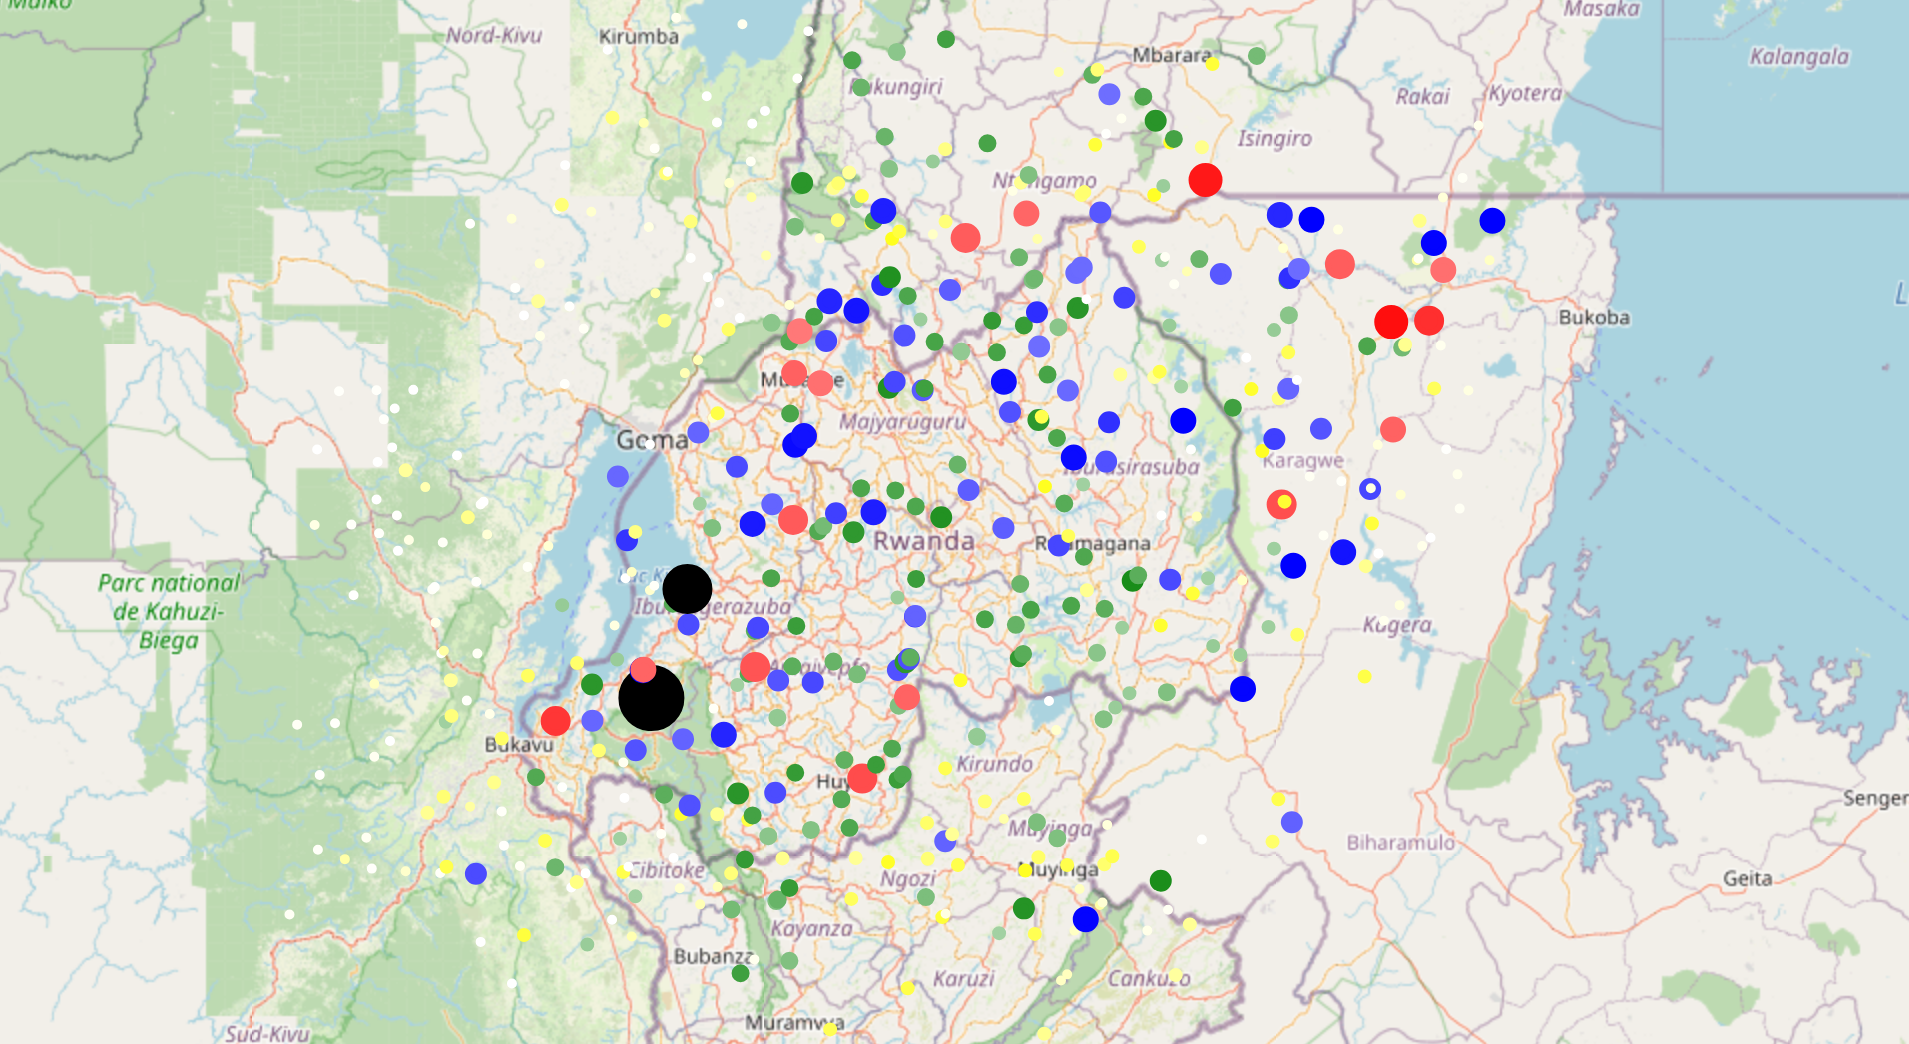
\includegraphics[width=1\textwidth]{output10.png}
      \caption{K聚类结果}
      \label{fig:10}
\end{figure}

\subsection{模型选择}

这是一个回归问题,我们尝试了多种回归模型,包括线性回归、支持向量回归、决策树回归、类别提升、自适应提升、极端梯度提升、随机森林、半径近邻、$K$ 近邻等。

\subsubsection{交叉验证}

交叉验证是一种评估模型性能的统计学方法。它的基本思想是将原始数据集分成两部分(训练集和验证集),然后在训练集上训练模型,在验证集上验证模型的性能。这个过程重复多次,每次都用不同的训练集和验证集,最后取平均值作为模型的最终性能。交叉验证的主要优点是它可以利用有限的数据获得模型在未知数据上的性能的更准确的估计。

在 Python 中,可以使用 \texttt{sklearn} 库的 \texttt{KFold} 函数进行交叉验证,以RF为例,代码如下:

\begin{lstlisting}[style=Python]
      from sklearn.model_selection import KFold
      rf_cv_scores = list()
      kf = KFold(n_splits=3, shuffle=True)
      for i, (train_ix, test_ix) in enumerate(kf.split(X)):
          X_train, X_test = X.iloc[train_ix], X.iloc[test_ix]
          Y_train, Y_test = y.iloc[train_ix], y.iloc[test_ix]
          rf_md = RandomForestRegressor().fit(X_train, Y_train)
          rf_pred = rf_md.predict(X_test)
          rf_score_fold = mean_squared_error(Y_test, rf_pred, squared=False)
          rf_cv_scores.append(rf_score_fold)
      print("RF Mean oof RMSE score is ==>", np.mean(rf_cv_scores))
\end{lstlisting}

\subsubsection{LinearRegression(线性回归)}

线性回归是一种预测模型,在这种模型中,我们假设目标变量和输入特征之间存在线性关系。这种关系可以用下面的数学公式表示:$y = a x + b$,其中,$y$ 是目标变量,$x$ 是输入特征,$a$ 和 $b$ 是模型的参数,它们定义了直线的斜率和截距。

在 Python 中,可以使用 \texttt{sklearn} 库的 \texttt{LinearRegression} 类来创建一个线性回归模型。我们调参比较后,最终选取特征为 \texttt{latitude}, \texttt{longitude}, \texttt{week\_no}, 对每个K聚类的结果分别进行线性回归并进行10折交叉验证,最后对预测结果乘以 1.06,最终得到 RMSE 为 44.9418298861089。

线性回归所产生的结果与其他模型相比较差,原因可能是:

\begin{itemize}
      \item 线性回归假设因变量和自变量之间存在线性关系。如果实际数据的关系是非线性的,那么线性回归的效果可能会不好。
      \item 如果自变量之间存在高度相关性或者异常值,那么可能会导致线性回归模型的不稳定,从而影响预测效果。
\end{itemize}

\subsubsection{SupportVectorRegressor(支持向量回归)}

支持向量回归是支持向量机在回归问题上的应用。它是一种强大的机器学习模型,可以用于解决非线性和高维度的回归问题。SVR 的基本思想是找到一个函数,使得该函数对于训练数据的预测值与真实值之间的误差最小,并且该函数的复杂度也要尽可能小。SVR 使用了一种叫做 ε-insensitive loss 的损失函数,这种损失函数只考虑预测值与真实值之间的误差大于 ε 的情况,小于 ε 的误差都被忽略。

我们先对整个训练集按照"latitude", "longitude", "week\_no", "emission", "k\_Means"的特征直接进行SVR,迭代次数 1000次,得到的结果为RMSE=196.52008720177972,并且即使在使用了 StandardScaler 或 MinMaxScaler 后,支持向量机均未能收敛,提示\texttt{ConvergenceWarning}。

因此,我们采用了对每个聚类分别进行支持向量回归并合并的方法,最终得到RMSE为57.84318401599136,并且仍然提示\texttt{ConvergenceWarning}。

支持向量回归的结果较差,原因可能是:

\begin{itemize}
      \item 支持向量回归对于异常值非常敏感。如果训练数据中包含很多异常值,那么支持向量回归可能会过度关注这些异常值,从而影响整体的预测性能。
      \item 支持向量回归有一些需要调整的参数,如惩罚系数 C 和核函数。如果这些参数没有设置得当,可能会影响支持向量回归的性能。
      \item 因此尝试使用其他的回归模型,如决策树回归或随机森林回归,这些模型可能对异常值更具鲁棒性。
\end{itemize}

\subsubsection{DecisionTreeRegressor(决策树回归)}

决策树回归使用决策树模型来进行连续值的预测,而不是像决策树分类那样预测离散的类标签。决策树回归的工作原理与决策树分类类似,都是通过一系列的问题来预测目标变量。但在决策树回归中,每个叶节点都代表一个预测值,这个预测值通常是所有到达该叶节点的数据点的目标变量值的平均值。

可以使用 \texttt{sklearn} 库中的 \texttt{DecisionTreeRegressor} 进行决策树回归。选择参数
\texttt{min\_samples\_leaf=3}, \texttt{min\_samples\_split=4},
选择特征 \texttt{latitude}, \texttt{longitude}, \texttt{year}, \texttt{week\_no}, \texttt{emission}, \texttt{k\_Means}, \texttt{rot\_30\_x},
进行 10 折验证,最终得到 RMSE 为 9.508541602900749。

\subsubsection{CatBoostRegressor(类别提升)}

CatBoost 是一个由 Yandex 开发的开源机器学习库,主要用于梯度提升决策树的训练。它可以自动处理分类特征,并防止过拟合。

我们仍然对每个聚类分别采用类别提升。

首先我们尝试默认参数下直接进行3折交叉验证,选取特征"latitude", "longitude", "week\_no", "emission", "k\_Means", "year",得到结果为RMSE=12.921159352568171。

我们认为欠拟合。于是更改参数learning\_rate=0.1, depth=10,得到RMSE=11.148340853326738。

\subsubsection{AdaBoostRegressor(自适应提升)}

自适应提升的工作原理是通过在一系列的弱学习器(例如,深度较浅的决策树)上应用权重,使得后续的模型更加关注在前一轮被错误分类的样本,从而提高整体模型的性能。它的自适应在于:前一个基本分类器被错误分类的样本的权值会增大,而正确分类的样本的权值会减小,并再次用来训练下一个基本分类器。同时,在每一轮迭代中,加入一个新的弱分类器,直到达到某个预定的足够小的错误率或达到预先指定的最大迭代次数才确定最终的强分类器。

选择特征 \texttt{latitude}, \texttt{longitude}, \texttt{year}, \texttt{week\_no}, \texttt{emission}, \texttt{rot\_30\_x}, \texttt{k\_Means},进行 10 折验证,最终得到 RMSE 为 49.007571729858626。

分析自适应提升的结果较差,原因可能是:

\begin{itemize}
      \item AdaBoost 对噪声数据和异常值非常敏感。如果训练数据中包含很多噪声数据或异常值,AdaBoost 可能会过度关注这些难以正确分类的样本,从而影响整体的预测性能。
      \item AdaBoost 有一些需要调整的参数,如弱学习器的数量和学习率。如果这些参数没有设置得当,可能会影响 AdaBoost 的性能。
      \item 尝试使用其他的集成学习方法,如随机森林或梯度提升,这些方法可能对噪声数据和异常值更具鲁棒性。
\end{itemize}

\subsubsection{XGBoostRegressor(极端梯度提升)}

极端梯度提升是一种优化的分布式梯度提升库,旨在实现高效、灵活和便携。它在许多机器学习竞赛和项目中都表现出色,因为它具有速度快和性能好的特点。

我们选取使用特征 \texttt{latitude}, \texttt{longitude}, \texttt{week\_no}, \texttt{k\_Means}, \texttt{year}, \texttt{rot\_30\_y}, \texttt{rot\_30\_x}, \texttt{rot\_15\_y}, \texttt{rot\_15\_x},共9个特征进行极端梯度提升,在3次交叉验证、结果乘以1.07后,RMSE能达到10.661617273590501。

\subsubsection{RandomForestRegressor(随机森林)}

随机森林通过构建并结合多个决策树来进行预测。随机森林的主要优点是它可以有效地处理大量的输入变量,并且不需要进行特征选择。此外,随机森林还具有很好的鲁棒性,并且可以有效地处理缺失数据和异常值。

我们使用了经纬度、年份、周数作为输入,参数设置 \texttt{min\_samples\_leaf=6},使用随机森林模型进行3折交叉验证训练,最终结果取乘以1.06,得到结果RMSE=5.04889854732325。

由于该模型与我们采用的测试集比对结果误差最小,我们在此特别地展示代码如下,其余模型代码不再展示:

\begin{lstlisting}[style=Python]
def RandomForestRegressor(self):
      train = self.train.loc[:, ["latitude", "longitude", "week_no", "emission", "year"]]
      test = self.test.loc[:, ["latitude", "longitude", "week_no", "year"]]
      X = train.drop(columns=["emission"])
      y = train["emission"].copy()

      rfr = RandomForestRegressor()
      rf_cv_scores = list()
      kf = KFold(n_splits=3, shuffle=True)
      for i, (train_ix, test_ix) in enumerate(kf.split(X)):
      X_train, X_test = X.iloc[train_ix], X.iloc[test_ix]
      Y_train, Y_test = y.iloc[train_ix], y.iloc[test_ix]
      rf_md = rfr.fit(X_train, Y_train)
      rf_pred = rf_md.predict(X_test)
      rf_score_fold = mean_squared_error(Y_test, rf_pred, squared=False)
      rf_cv_scores.append(rf_score_fold)
      print("RF Mean oof RMSE score is ==>", np.mean(rf_cv_scores))

      rfr.fit(X, y)
      rfr_pred = rfr.predict(test)
      test["emission"] = rfr_pred * 1.06
      self.ans = test.loc[:, ["emission"]]
\end{lstlisting}

\subsubsection{KNeighborsRegressor(K近邻)}

$k$-近邻是一种基于实例的学习或非参数懒惰学习的方法。它的工作原理是,对于一个新的输入实例,算法会在训练数据集中找到与其最近的 $k$ 个实例(即 $k$ 个邻居),然后根据这些邻居的标签来预测新实例的标签。

我们调参后选取n\_neighbors=3,并进行3折交叉验证,最终得到RMSE为14.318270658110539。

\subsubsection{RadiusNeighborsRegressor(半径近邻)}

半径近邻类似于 $k$-近邻,但有一个关键的区别:在 $k$-近邻算法中,我们选择最近的 $k$ 个点并根据它们的标签来预测新点的标签。然而,在半径近邻中,我们选择在给定半径内的所有点,并根据它们的标签来预测新点的标签。

我们选取"latitude", "longitude", "week\_no", "emission"为特征,进行radius=0的半径近邻回归,最后对结果乘以1.07,得到的结果为RMSE=14.318270658110535。

需要说明的是,半径近邻无法使用year作为特征,因为year是离散值,而半径近邻只能处理连续值。同时,也无法进行交叉验证,因为半径近邻无法处理离散值。

可以看出,半径近邻的结果与K近邻最优结果基本一致,因为他们的基本思想是相同的。这两种方法不需要过多调参,但同时也导致了优化空间较小。

\subsection{结果优化}

显然,预测出的CO2排放量不可能为负数,因此我们将预测出的负数值置为 0。

除此之外,我们相信训练集的数据中,如果某个地点在 2019-2021 年的 CO2 排放量均为 0,那么这个地点在2022年的CO2排放量也应该为 0 。因此,我们将这些地点的预测值置为 0。

代码如下:

\begin{lstlisting}[style=Python]
      y_pred[y_pred < 0] = 0
      
      zero_emissions = train.groupby(['latitude', 'longitude'])['emission'].mean().to_frame()
      zero_emissions = zero_emissions[zero_emissions['emission'] == 0]
      mask = test.apply(lambda x: (x['latitude'], x['longitude']) in zero_emissions.index, axis=1)
      y_pred.loc[mask, "emission"] = 0
\end{lstlisting}

处理后对评估结果(RMSE)有一定的提升。

\section{评估}

\subsection{RMSE}

在 Python 中,我们选取 \texttt{sklearn} 库的 \texttt{mean\_squared\_error} 函数计算 RMSE,代码如下:

\begin{lstlisting}[style=Python]
      rmse = mean_squared_error(test["emission"], ans["emission"], squared=False)
\end{lstlisting}

\subsection{最终得分}

由于kaggle中该比赛从2023年8月1日开始,2023年8月22日结束,在本次工作进行时,kaggle已经关闭了提交通道,因此我们无法得到准确得分。我们将采用与高分答案的对比来评估我们的模型。我们选取的对比答案是来自于kaggle中private数据集排名第三队伍public部分的答案,其private部分得分为9.43672。链接为\href{https://www.kaggle.com/competitions/playground-series-s3e20/discussion/433822}{3rd Place Solution}。

最终我们决定使用RandomForestRegressor(随机森林)模型所产生的结果,它与对比答案的RMSE为5.04889854732325。

\subsection{预测结果可视化}

我们将2019-2021的训练数据与2021-2022的预测数据按照每日总排放量绘制到同一张图中,进行预测结果可视化,如图\ref{fig:13} 所示。

\begin{figure}[H]
      \centering
      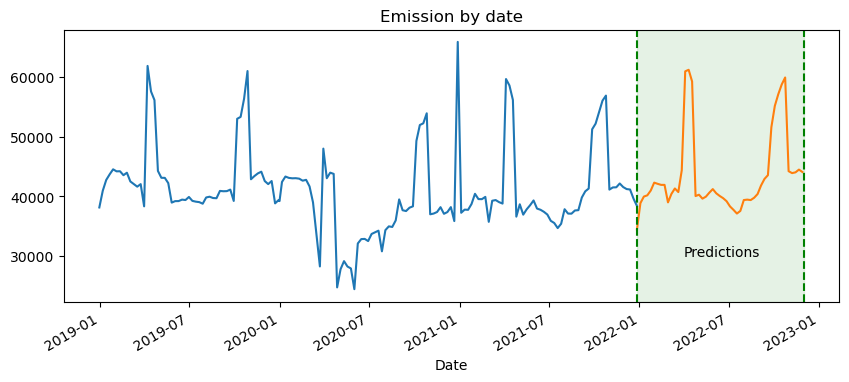
\includegraphics[width=1\textwidth]{output13.png}
      \caption{预测结果可视化}
      \label{fig:13}
\end{figure}

\section{团队成员分工}

\subsection{吕思翰}

TODO

\subsection{来泽远}

主要负责初版代码与再版框架的编写、关于时间和空间的特征工程、量化分析、异常值处理、K聚类、部分模型编写,参与了文档撰写和大部分其他工作。

\subsection{曹宸瑞}

主要负责方法调研、缺失值处理、数据归一化、气象数据与其他特征分析、交叉验证、大部分模型选择与比较、撰写文档框架,参与了文档撰写和大部分其他工作。

\section{总结与感悟}

在本次实验中,我们学习了数据科学的基本流程,包括数据分析、数据预处理、特征工程、模型选择、模型评估等。

我们实践了特征工程,包括特征提取、特征选择、特征变换;接触了多种机器学习模型,例如线性回归、支持向量机、决策树、随机森林、AdaBoost、XGBoost等或经典或新兴的模型,并对其进行调参、交叉验证与比较。我们学习了如何使用 Python 进行数据分析和机器学习,对于 Python 也有了更深入的了解。我们学会了如何对数据进行基本处理,如何使用 Kaggle 平台进行数据科学竞赛,如何使用 \LaTeX{} 进行文档排版。同时,通过阅读他人的代码和解决方案,我们了解了很多不同的思路和方法。我们与队友一起合作、交流和分享想法,学习了更多关于团队合作和沟通的技巧。

\ctexset{bibname=参考资料}
\begin{thebibliography}{100}
      \bibitem{ref1}\href{https://www.kaggle.com/code/ambrosm/pss3e20-eda-which-makes-sense}{PSS3E20 EDA which makes sense}
      \bibitem{ref2}\href{https://www.kaggle.com/code/kacperrabczewski/rwanda-co2-step-by-step-guide}{Rwanda CO2: Step by step guide}
      \bibitem{ref3}\href{https://www.kaggle.com/code/yaaangzhou/pg-s3-e20-eda-modeling}{[PG S3 E20] EDA + Modeling}
      \bibitem{ref4}\href{https://www.kaggle.com/code/dmitryuarov/ps3e20-rwanda-emission-advanced-fe-20-88}{PS3E20 | Rwanda emission | Advanced FE | 20.88}
\end{thebibliography}

\end{document}
